
\begin{figure}[h]
%\label{fig:N9}
\scalebox{.5}{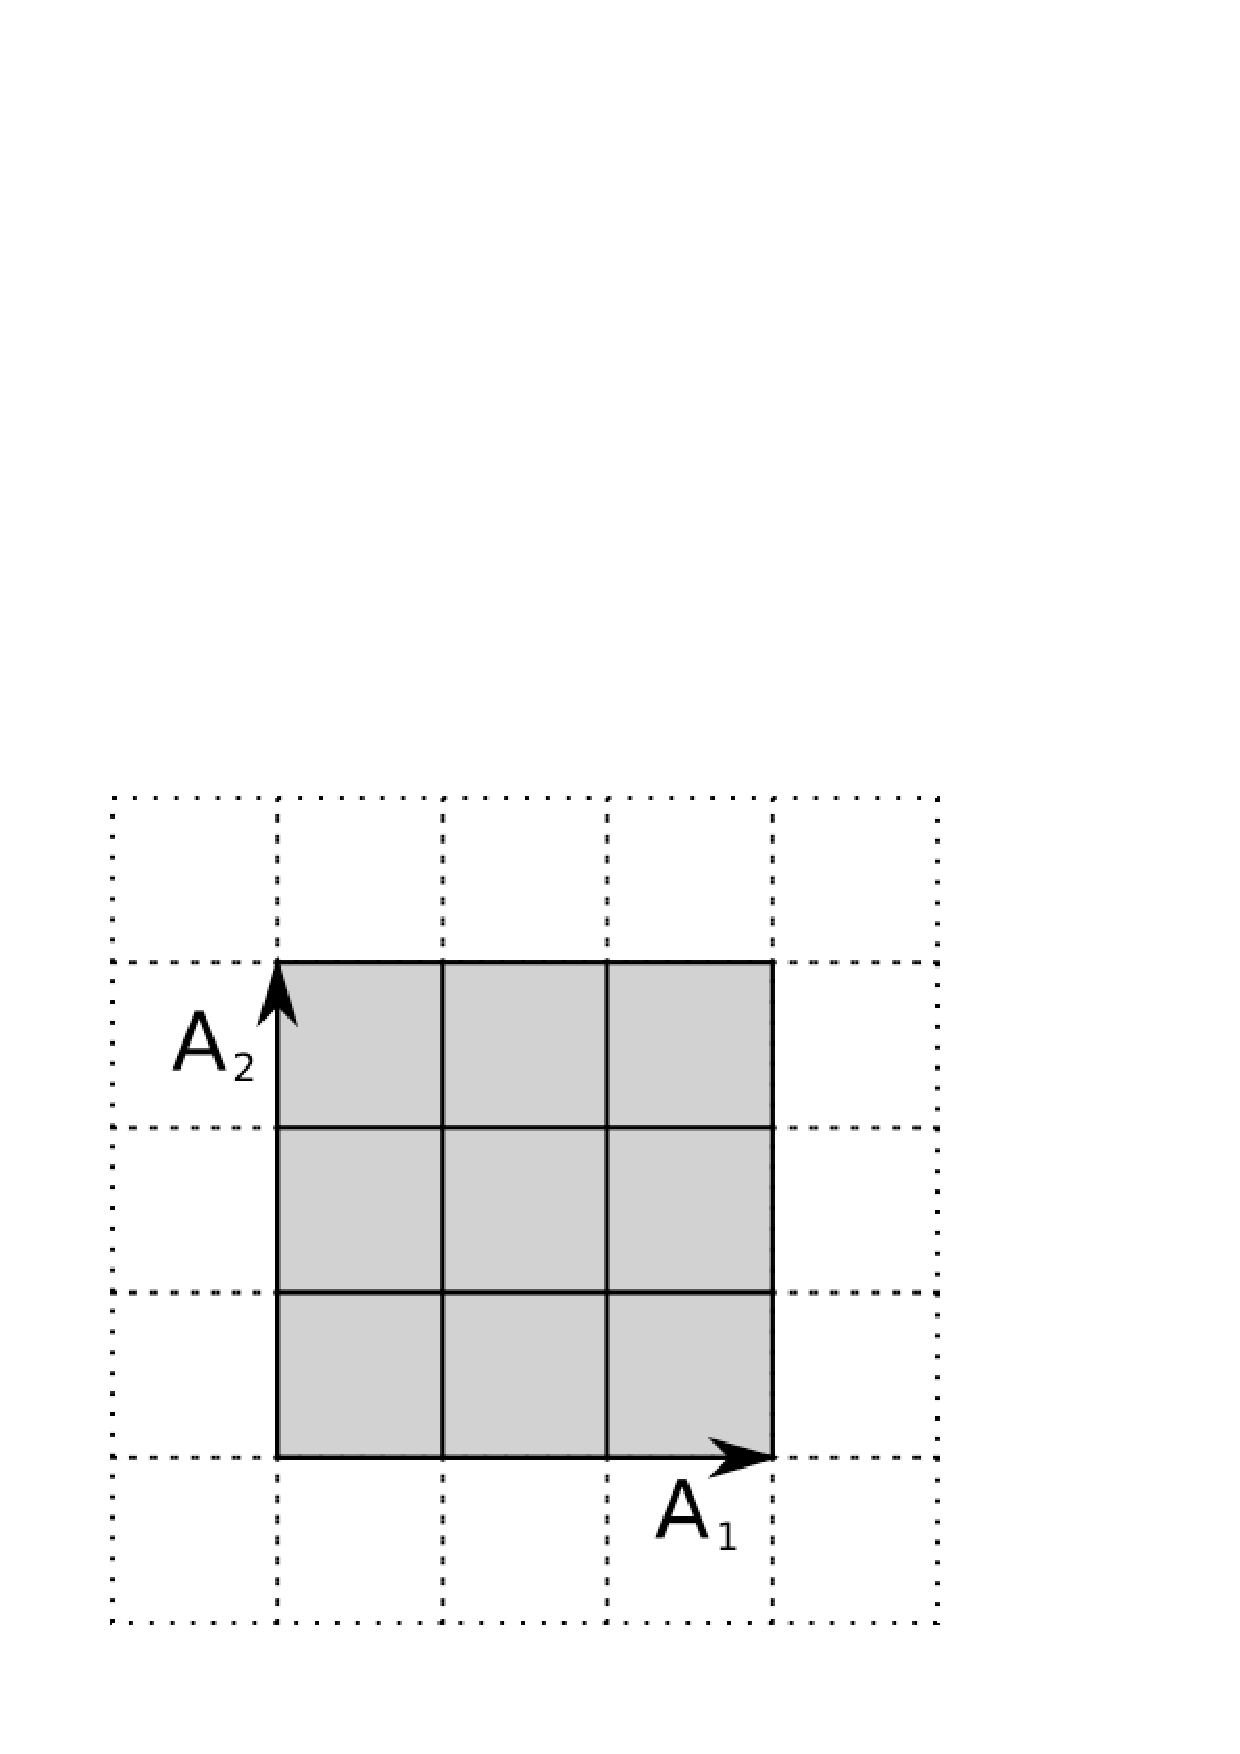
\includegraphics{figures/3x3.pdf}}
\caption{\label{fig:N9} An example of a perfect square packing with density 1: $N=9$.}
\end{figure}

\begin{figure}[H]

\scalebox{.4}{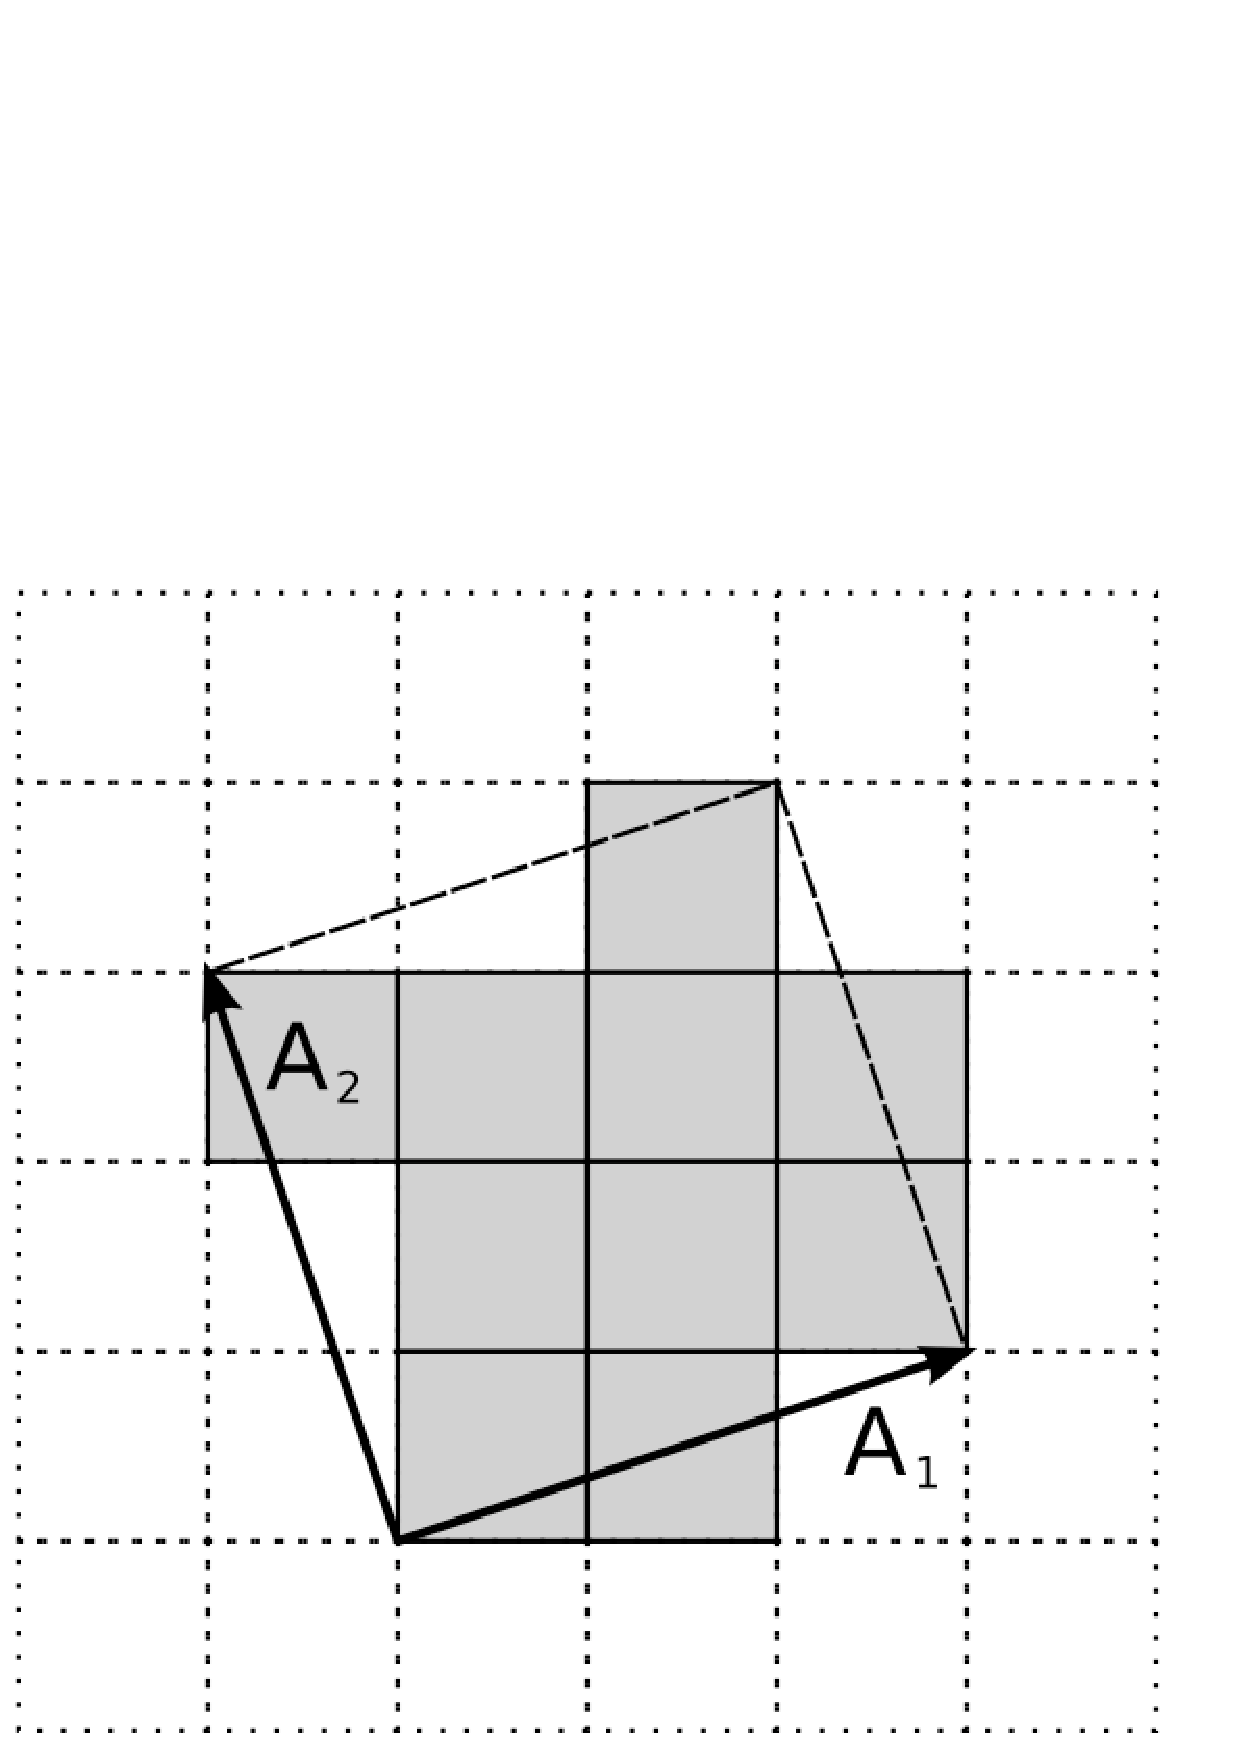
\includegraphics{figures/bravais1.pdf}}
\caption{\label{fig:bravais}An example of a packing for which $N$ is equal to the sum of two squares: $N=10$; all such packings are density $1$.}
\end{figure}

\begin{figure}[H]

\scalebox{.4}{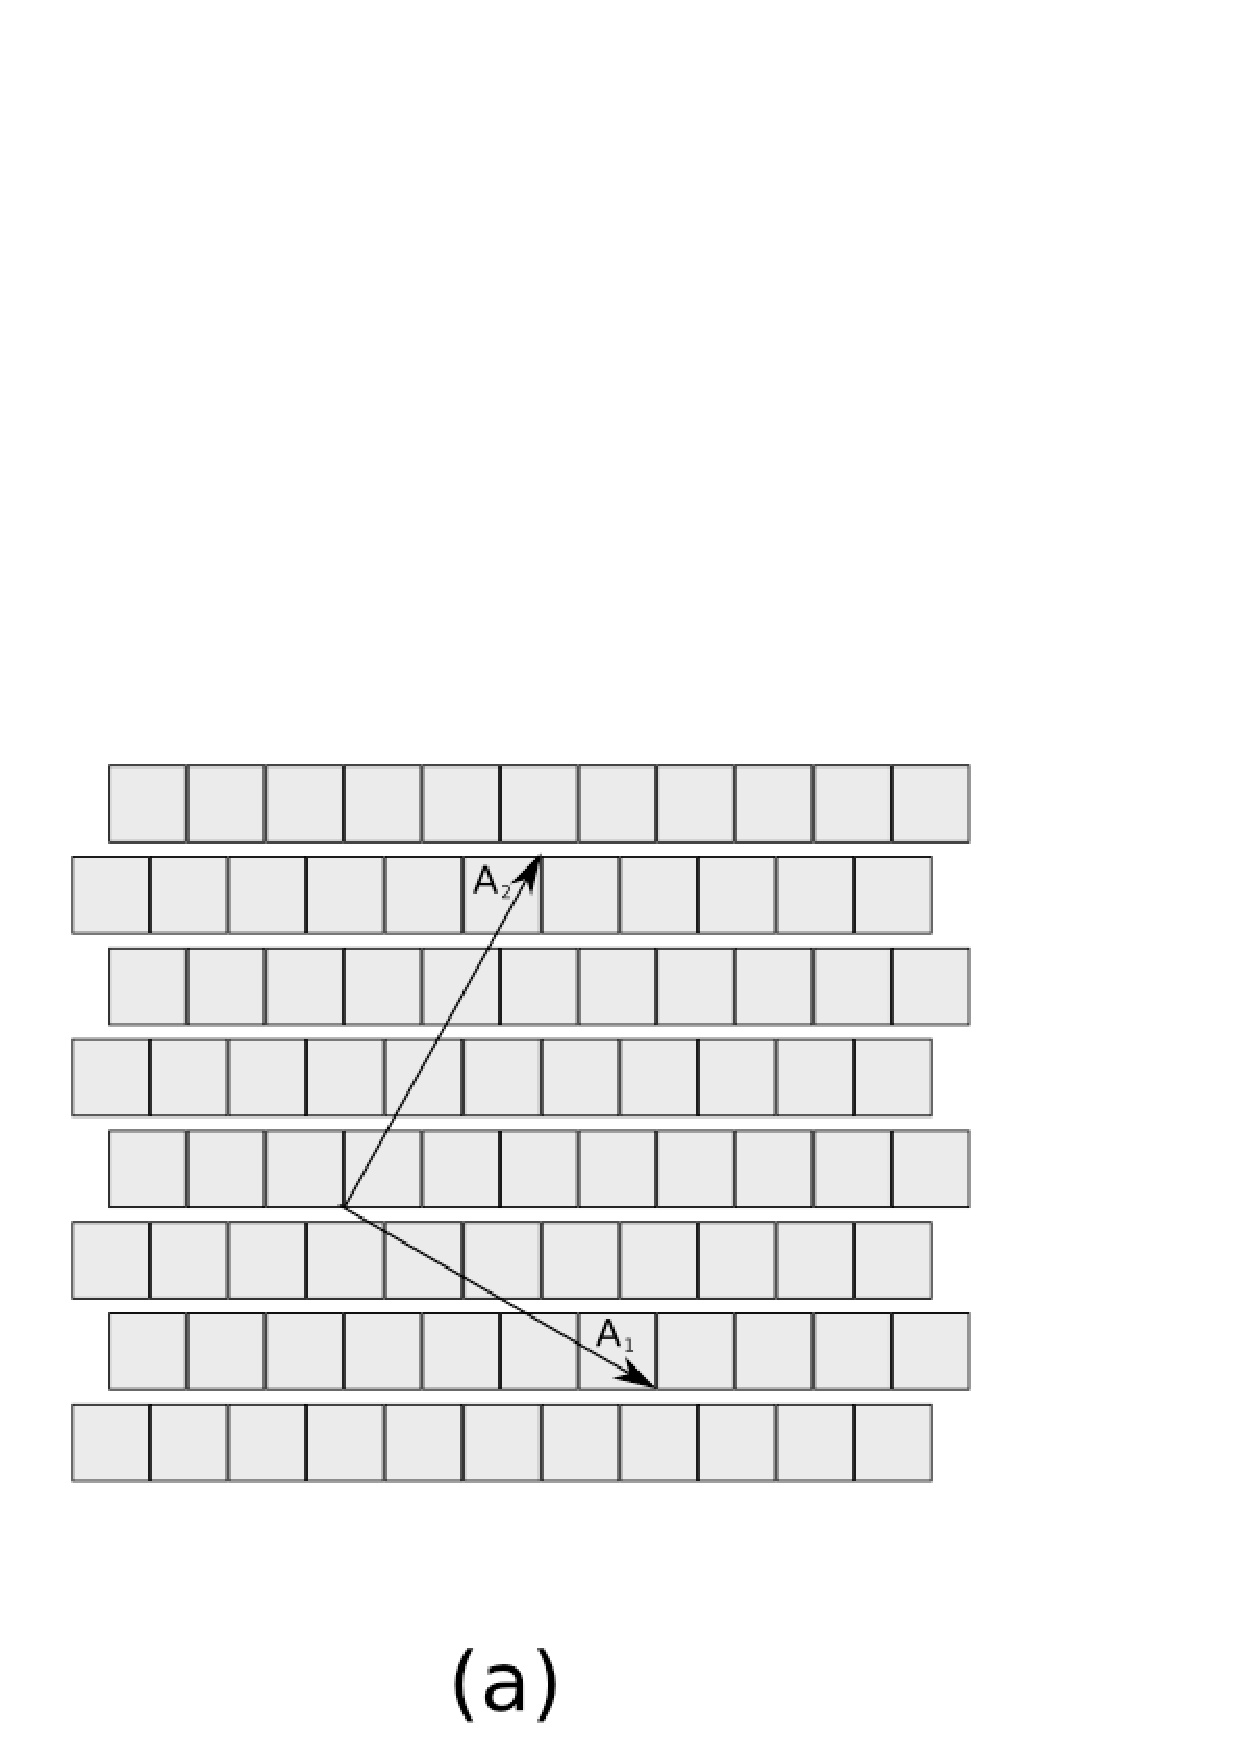
\includegraphics{figures/gappedCombo1.pdf}}
\caption{\label{fig:gb}Schematic (a) of a ``gapped bricklayer'' configuration, with density $\rho = (N-1)/N$. Results of simulated annealing for $N=11$ are shown in (b).}
\end{figure}

\begin{figure}[H]

\scalebox{.45}{\includegraphics{figures/N22.pdf}}
\caption{\label{fig:n22}Simulation results for $N=22$: the conjectured best packing is a ``gapped bricklayer with domino bricks''.}
\end{figure}


\begin{figure}[H]
\scalebox{.25}{\includegraphics{figures/N12.pdf}}
\caption{\label{fig:n12}Simulation results for $N=12$: a lattice of $\frac{1}{2} \times \frac{1}{2}$ holes.}
\end{figure}

\begin{figure}[H]
\scalebox{.35}{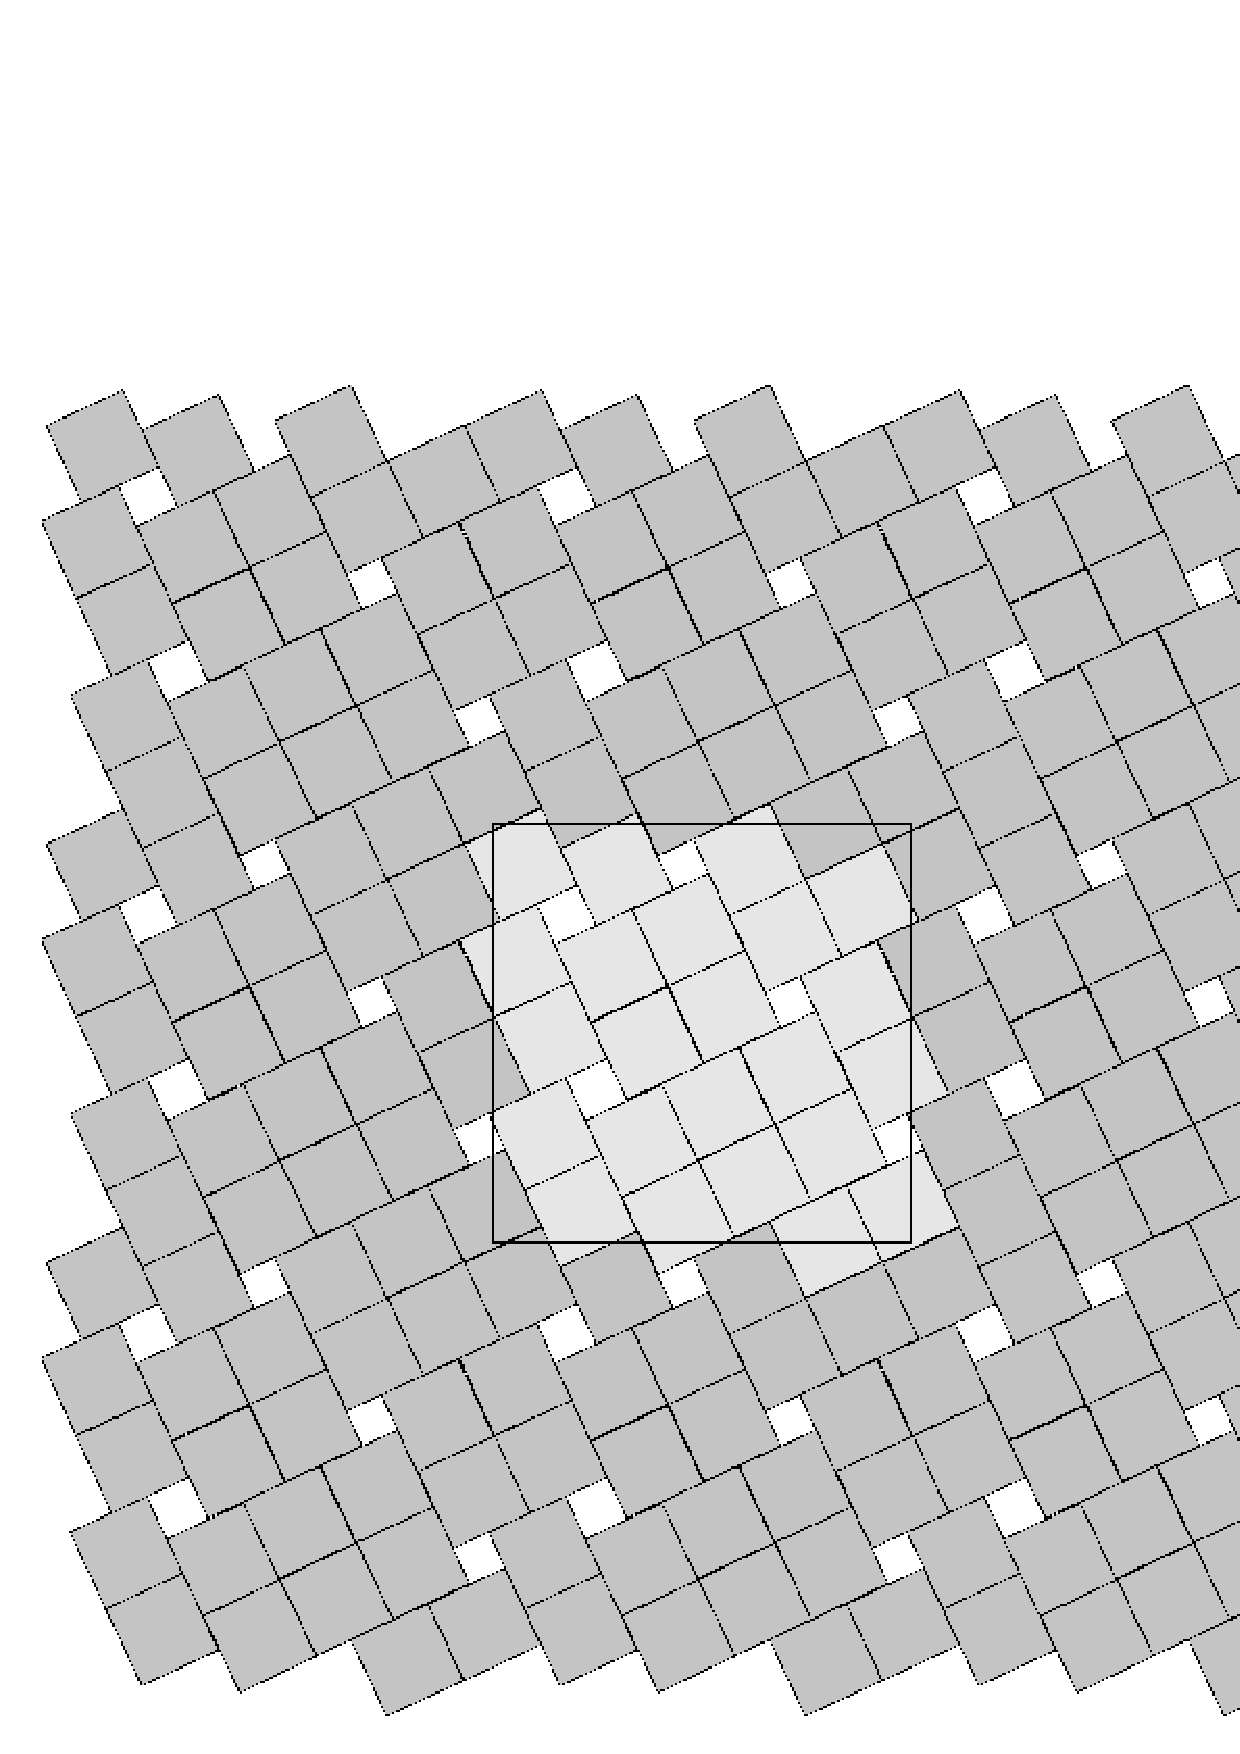
\includegraphics{figures/N23.pdf}}
\caption{\label{fig:n23}Simulation results for $N=23$: a lattice of $\frac{1}{2} \times \frac{1}{2}$ holes.}
\end{figure}

\begin{figure}[H]
\scalebox{.3}{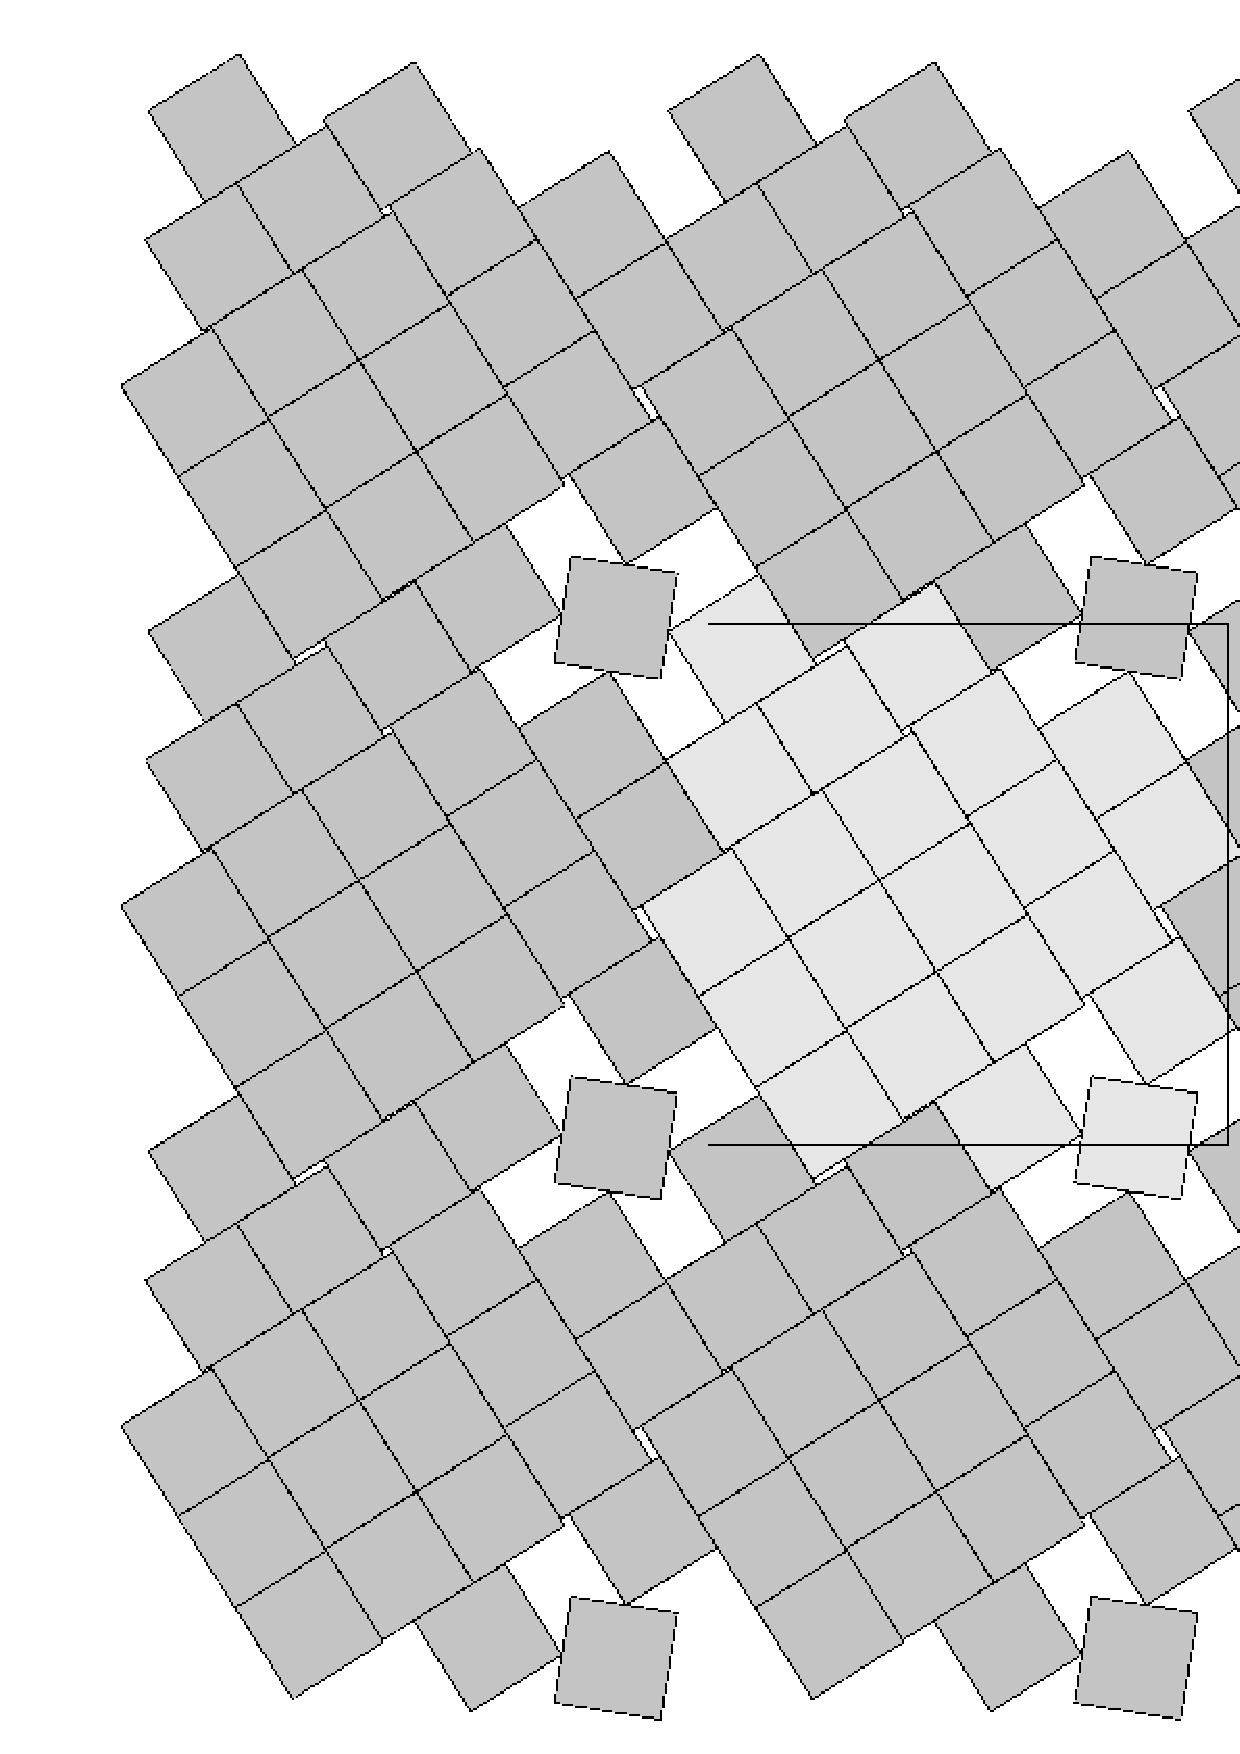
\includegraphics{figures/N21.pdf}}
\caption{\label{fig:n21}Simulation results for $N=21$: a lattice of skew squares embedded in a square lattice.  The $5$-square pattern (which includes a skew square in its center) is the proved best packing of 5 squares in a square \cite{Friedman2002}. Note that the simulation results have not yet converged to the conjectured best packing configuration.}
\end{figure}

\begin{figure}[H]
\scalebox{.3}{\includegraphics{figures/alignedBlocks.pdf}}
\caption{\label{fig:aligned}}
\end{figure}

\begin{figure}[H]
\scalebox{.3}{\includegraphics{figures/pythagoras.pdf}}
\caption{\label{fig:pythagoras}}
\end{figure}


\begin{figure}[H]
\scalebox{.4}{\includegraphics{figures/Bezout1.pdf}}
\caption{\label{fig:Bezout}}
\end{figure}
